\Opensolutionfile{ans}[ans/ansBTOTC1]
%%=====Câu 1
\begin{ex}%Câu 1%[0D1Y1-1]
	Trong các phát biểu sau, phát biểu nào là mệnh đề?
	\choice
	{\True $3$ là số tự nhiên}
	{Mấy giờ rồi!}
	{Các em hãy cố gắng học tập!}
	{Ngày mai bạn có đi du lịch không?}
	\loigiai{
		``$3$ là số tự nhiên'' là mệnh đề.
	}
\end{ex}

%%=====Câu 2
\begin{ex}%[0D1Y1-1]
	Cho các câu sau đây:
	\begin{enumerate}
		\item ``Phan-xi-păng là ngọn núi cao nhất Việt Nam''.
		\item ``$\pi^2<9,86$''.
		\item ``Mệt quá!''.
		\item ``Chị ơi, mấy giờ rồi?''.
	\end{enumerate}
	Hỏi có bao nhiêu câu là mệnh đề?
	\choice
	{$1$}
	{$3$}
	{$4$}
	{\True $2$}
	\loigiai{
		Các khẳng định sau là mệnh đề ``Phan-xi-păng là ngọn núi cao nhất Việt Nam'', ``$\pi^2<9,86$''.
	}
\end{ex}
%%=====Câu 3
\begin{ex}%Câu 1%[0D1Y1-1]
	Xét các phát biểu sau:
	\begin{itemize}
		\item Sài Gòn là thủ đô Việt Nam.
		\item Một giờ có 60 phút.
		\item Sao nóng thế này?
		\item Thật tuyệt vời!
	\end{itemize}
	Có bao nhiêu mệnh đề trong các phát biểu trên?
	\choice
	{$1$}
	{\True $2$}
	{$3$}
	{$4$}
	\loigiai{
		Các mệnh đề: ``Sài Gòn là thủ đô Việt Nam'', ``Một giờ có 60 phút''.
	}
\end{ex}

%%=====Câu 4
\begin{ex}%[0D1Y1-1]
	Có bao nhiêu mệnh đề chứa biến trong các phát biểu sau
	\begin{itemize}
		\item $x+y=2$.
		\item $2+n$ chia hết cho $2$.
		\item $\pi -3 =0$.
		\item $n$ là số tự nhiên.
	\end{itemize}
	\choice
	{$0$}
	{$1$}
	{$2$}
	{\True $3$}
	\loigiai{
		Có $3$ mệnh đề chứa biến là $x+y=2$, $2+n$ chia hết cho $2$, $n$ là số tự nhiên.
	}
\end{ex}

%%=====Câu 5
\begin{ex}%[0D1Y1-1]
	Trong các câu sau, có bao nhiêu câu là mệnh đề
	\begin{enumerate}
		\item Huế là một thành phố của Việt Nam.
		\item Sông Hương chảy ngang qua thành phố Huế.
		\item Hãy trả lời câu hỏi này!
		\item $5+19-24$.
		\item $6+81=25$.
		\item Bạn có rỗi tối nay không?
		\item $x+2=11$.
	\end{enumerate}
	\choice
	{$1$}
	{$2$}
	{\True $3$}
	{$4$}
	\loigiai{
		Mệnh đề là: Huế là một thành phố của Việt Nam, Sông Hương chảy ngang qua thành phố Huế, $6+81=25$.
	}
\end{ex}
\begin{ex}%[0D1Y1-1]
	Trong các câu sau câu nào là một mệnh đề?
	\choice
	{\True $11$ là một số nguyên tố}
	{Hôm nay trời đẹp quá!}
	{Ngày mai bạn có đi học không?}
	{Mấy giờ rồi?}
	\loigiai{
		Mệnh đề: $13$ là một số nguyên tố.
	}
\end{ex}
\begin{ex}%[0D1Y1-1]
	Phát biểu nào sau đây là mệnh đề?
	\choice
	{Đề trắc nghiệm môn Toán năm nay dễ quá!}
	{Cấm học sinh quay cóp trong kiểm tra}
	{\True Toán học là một môn thi trong kỳ thi THPT Quốc Gia}
	{Bạn biết câu nào là đúng không?}
	\loigiai{
		Toán học là một môn thi trong kỳ thi THPT Quốc Gia: Đây là mệnh đề.
	}
\end{ex}

\begin{ex}%[0D1B1]
Trong các câu khẳng định sau, câu nào là mệnh đề \textbf{sai}?
\choice
{\True Nếu tam giác $ABC$ thỏa mãn $AB^2+AC^2=BC^2$ thì tam giác $ABC$ vuông tại $B$}
{2 là số nguyên tố}
{Nếu một phương trình bậc hai có biệt thức $\Delta$ không âm thì nó có nghiệm}
{Tổng $3$ góc trong của một tam giác bằng $180^0$} 
\loigiai{
Mệnh đề sai là mệnh đề \lq\lq Nếu tam giác $ABC$ thỏa mãn $AB^2+AC^2=BC^2$ thì tam giác $ABC$ vuông tại $B$\rq\rq.
}
\end{ex}
\begin{ex}%[0D1B1]
Trong các mệnh đề sau, mệnh đề nào \textbf{sai}?
\choice
{Nếu $n$ là một số nguyên lẻ thì $n^2$ là số lẻ}
{Điều kiện cần và đủ để số tự nhiên $n$ chia hết cho 3 là tổng các chữ số của nó chia hết cho $3$}
{\True Tứ giác $ABCD$ là hình chữ nhật khi và chỉ khi nó thỏa mãn $AC=BD$}
{Tam giác $ABC$ là tam giác đều khi và chỉ khi nó thỏa mãn đồng thời hai điều kiện $AB=AC$ và $\widehat{A}=60^0$} 
\loigiai{
Mệnh đề sai là mệnh đề \lq\lq Tứ giác $ABCD$ là hình chữ nhật khi và chỉ khi nó thỏa mãn $AC=BD$\rq\rq.
}
\end{ex}

\begin{ex}%[Phạm Quang Tú]%[0D1B1]
Trong các mệnh đề sau, mệnh đề nào đúng?
\choice
{Nếu $a\ge b$ thì $a^2\ge b^2$}
{Nếu $a^2 \ge b^2$ thì $a \ge b$}
{\True Nếu $a$ chia hết cho $9$ thì $a$ chia hết cho $3$}
{Nếu $a$ chia hết cho 3 thì $a$ chia hết cho $9$}
\loigiai{
Mệnh đề đúng là mệnh đề \lq\lq Nếu $a$ chia hết cho $9$ thì $a$ chia hết cho $3$\rq\rq.
}
\end{ex}


\begin{ex}%[0D1B1] 
Biết $A$ là mệnh đề sai, còn $B$ là mệnh đề đúng. Mệnh đề nào sau đây đúng?
\choice 
{ $B\Rightarrow A$}
{ $B\Leftrightarrow A$ }
{ $\overline{A}\Leftrightarrow \overline{B}$ }
{ \True $B\Rightarrow \overline{A}$} 
\loigiai{
Mệnh đề đúng là mệnh đề \lq\lq $B\Rightarrow \overline{A}$\rq\rq.
}
\end{ex} 
\begin{ex}%[Phạm Quang Tú]%[0D1B1]
Cho $a,b$ là hai số tự  nhiên. Mệnh đề nào sau đây \textbf{sai}?
\choice
{Nếu $a, b$ là các số lẻ thì $ab$ lẻ}
{\True Nếu $a$ chẵn và $b$ lẻ thì $ab$ lẻ}
{Nếu $a$ và $b$ lẻ thì $a+b$ chẵn}
{Nếu $a^2$ lẻ thì $a$ lẻ} 
\loigiai{
Mệnh đề sai là mệnh đề \lq\lq Nếu $a$ chẵn và $b$ lẻ thì $ab$ lẻ\rq\rq.
}
\end{ex}

\begin{ex}%[Phạm Quang Tú]%[0D1B1]
Trong các mệnh đề sau, mệnh đề nào \textbf{sai}?
\choice
{\True Nếu $m,n$ là các số vô tỉ thì $m.n$ cũng là số vô tỉ}
{Nếu $ABC$ là một tam giác vuông thì đường trung tuyến ứng với cạnh huyền bằng nửa cạnh huyền}
{Với ba vectơ $\overrightarrow{a},\overrightarrow{b},\overrightarrow{c}$ đều khác vectơ $\overrightarrow{0}$, nếu $\overrightarrow{a},\overrightarrow{b}$ cùng hướng với $\overrightarrow{c}$ thì $\overrightarrow{a},\overrightarrow{b}$ cùng hướng}
{Điểm $G$ là trọng tâm của tam giác $ABC$ khi và chỉ khi $\overrightarrow{GA}+\overrightarrow{GB}+\overrightarrow{GC}=\overrightarrow{0}$}
\loigiai{
Mệnh đề sai là mệnh đề \lq\lq Nếu $m,n$ là các số vô tỉ thì $m.n$ cũng là số vô tỉ\rq\rq.
}
\end{ex}

\begin{ex}
Cho các mệnh đề $ P:$ “$5$ chia hết cho $2$” và $Q:$ ”$11$ là số nguyên tố”. Tìm mệnh đề đúng trong các mệnh đề sau.
\choice
{$Q \Rightarrow P$}
{$\overline{P} \Rightarrow \overline{Q}$}
{$P \Leftrightarrow Q$}
{\True $P \Rightarrow Q$}
\loigiai{
Mệnh đề đúng là mệnh đề \lq\lq $P \Rightarrow Q$\rq\rq.
}
\end{ex}

\begin{ex}%[Trần Ngọc Lam]%[0D1B1] 
Xét mệnh đề chứa biến $P(n):$ “$n$ chia hết cho $12$”. Mệnh đề nào dưới đây đúng?
\choice 
{\True $P(48)$} 
{ $P(4) $} 
{ $P(3)$} 
{ $P(88)$}
\loigiai{
Mệnh đề đúng là \lq\lq $P(48)$\rq\rq.
}
\end{ex}

\begin{ex}%[Phạm Quang Tú]%[0D1K1]
Trong các câu sau, có bao nhiêu câu là mệnh đề? Có bao nhiêu mệnh đề đúng?
\begin{enumerate}
\item Tam giác cân có hai góc bằng nhau phải không?
\item Hai vectơ có độ dài bằng nhau thì bằng nhau.
\item Một tháng có tối đa 5 ngày chủ nhật.
\item $23$ là một số nguyên tố.
\item Đồ thị của hàm số $y=ax^2(a \neq 0)$ là một đường parabol.
\end{enumerate}
\choice
{Có $5$ mệnh đề; $4$ mệnh đề đúng}
{\True Có $4$ mệnh đề; $3$ mệnh đề đúng}
{Có $3$ mệnh đề; $2$ mệnh đề đúng}
{Có $4$ mệnh đề; $2$ mệnh đề đúng}
\loigiai{
\begin{enumerate}
	\item \lq\lq Tam giác cân có hai góc bằng nhau phải không?\rq\rq\, không phải là mệnh đề.
	\item \lq\lq Hai vectơ có độ dài bằng nhau thì bằng nhau.\rq\rq\, là một mệnh đề sai.
	\item \lq\lq Một tháng có tối đa 5 ngày chủ nhật.\rq\rq\, là một mệnh đề đúng.
	\item \lq\lq $23$ là một số nguyên tố.\rq\rq\, là mệnh đề đúng.
	\item \lq\lq Đồ thị của hàm số $y=ax^2(a \neq 0)$ là một đường parabol.\rq\rq\, nếu mệnh đề đúng.
\end{enumerate}
Vậy có $4$ mệnh đề; $3$ mệnh đề đúng.
}
\end{ex}
\begin{ex}%[Trần Ngọc Lam]%[0D1K1] 
Trong các mệnh đề sau, mệnh đề nào \textbf{sai} ?
\choice 
{ \True $-\pi <-2\Leftrightarrow {{\pi }^2}<4$}
{ $\pi <4\Leftrightarrow {{\pi }^2}<16$} 
{ $\sqrt{23}<5\Rightarrow 2\sqrt{23}<2\cdot5$}
{ $\sqrt{23}<5\Rightarrow -2\sqrt{23}>-2\cdot5$}
\loigiai{
Mệnh đề sai là mệnh đề \lq\lq $-\pi <-2\Leftrightarrow {{\pi }^2}<4$\rq\rq.
}
\end{ex} 
\begin{ex}%[Trần Ngọc Lam]%[0D1K1] 
Mệnh đề nào dưới đây đúng?
\choice 
{ $\pi$ là số không nhỏ hơn 4} 
{ Nếu $a, b, c, d$ là các số thực thỏa mãn $a+b>c+d$ thì $a>c$ và $b>d$} 
{ \True Nếu $a>3$ thì $a>0$} 
{ $\exists x\in \mathbb{N},x^2=2$ }
\loigiai{
Mệnh đề đúng là mệnh đề \lq\lq Nếu $a>3$ thì $a>0$\rq\rq.
}
\end{ex}

\begin{ex}%[Phạm Quang Tú]%[0D1G1]
Tìm mệnh đề đúng trong các mệnh đề sau.
\choice
{Một năm có tối đa $52$ ngày chủ nhật}
{Các số nguyên tố đều là số lẻ}
{Giải thưởng lớn nhất của Toán học là giải Nobel}
{\True Có vô số số nguyên tố}
\loigiai{
Mệnh đề đúng là mệnh đề \lq\lq Có vô số số nguyên tố\rq\rq.
}
\end{ex}

%%=====Câu 1
\begin{ex}%[Ngân hàng tex khối 10-lần 1]%[0D1Y1-3]
	Cho mệnh đề ``Có một học sinh trong lớp $A_1$ không chấp hành luật giao thông''. Mệnh đề phủ định của mệnh đề này là mệnh đề nào sau đây?
	\choice
	{Không có học sinh nào trong lớp $A_1$ chấp hành luật giao thông}
	{\True Mọi học sinh trong lớp $A_1$ đều chấp hành luật giao thông}
	{Có một học sinh trong lớp $A_1$ chấp hành luật giao thông}
	{Mọi học sinh trong lớp $A_1$ không chấp hành luật giao thông}
	\loigiai
	{
		Mệnh đề phủ định của mệnh đề ``Có một học sinh trong lớp $A_1$ không chấp hành luật giao thông'' là mệnh đề ``Mọi học sinh trong lớp $A_1$ đều chấp hành luật giao thông''.
	}
\end{ex} 

%%=====Câu 2
\begin{ex}%[Ngân hàng tex khối 10-lần 1]%[0D1Y1-3]
	Mệnh đề phủ định của mệnh đề “$2019$ là số tự nhiên lẻ” là
	\choice
	{$2019$ là số tự nhiên lẻ}
	{$2019$ là số nguyên tố}
	{\True $2019$ không là số tự nhiên lẻ}
	{$2019$ là số chính phương}
	\loigiai{
		Mệnh đề phủ định của mệnh đề “$2019$ là số tự nhiên lẻ” là “$2019$ không là số tự nhiên lẻ”. }
\end{ex}

%%=====Câu 3
\begin{ex}%[Ngân hàng tex khối 10-lần 1]%[0D1Y1-3]
	Mệnh đề nào sau đây là phủ định của mệnh đề  \lq\lq Mọi người đều phải đi làm \rq\rq?
	\choice
	{Có một người đi làm}
	{Tất cả đều phải đi làm}
	{\True Có ít nhất một người không đi làm}
	{Mọi người đều không đi làm}
	\loigiai{
		Phủ định của mệnh đề đã cho là \lq\lq  Có ít nhất một người không đi làm\rq\rq.
	}
\end{ex}

%%=====Câu 4
\begin{ex}%[Ngân hàng tex khối 10-lần 1]%[0D1Y1-3]
	Mệnh đề nào dưới đây là mệnh đề phủ định của mệnh đề “$2$ là số nguyên tố”?
	\choice
	{$2$ là số nguyên dương}
	{$2$ là số nguyên âm}
	{\True $2$ không phải là số nguyên tố}
	{$2$ là số không nguyên}
	\loigiai{
		Theo định nghĩa, ta có mệnh đề phủ định của mệnh đề “$2$ là số nguyên tố" là mệnh đề “$2$ không phải là số nguyên tố”.
	}
\end{ex}
%%=====Câu 5
\begin{ex}%[Ngân hàng tex khối 10-lần 1]%%[0D1Y1-3]
	Lập mệnh đề phủ định của mệnh đề: “ Số 6 chia hết cho 2 và 3”.
	\choice 
	{ Số 6 chia hết cho 2 hoặc 3} 
	{ Số 6 không chia hết cho 2 và 3} 
	{ \True Số 6 không chia hết cho 2 hoặc 3} 
	{ Số 6 không chia hết cho 2 và chia hết cho 3} 
	\loigiai { 
		Phủ định của mệnh đề “ Số 6 chia hết cho 2 và 3” là mệnh đề: “Số 6 không chia hết cho 2 hoặc 3”}
\end{ex}
%6
\begin{ex}%[Ngân hàng tex khối 10-lần 1]%[0D1Y1-3]
	Cho mệnh đề "Phương trình  $x^2+2x+1=0$ có nghiệm". Tìm mệnh đề phủ định của mệnh đề trên và cho biết tính đúng sai của mệnh đề phủ định.
	\choice 
	{``Phương trình $x^2+2x+1=0$ có hai nghiệm phân biệt''. Đây là mệnh đề sai}
	{``Phương trình $x^2+2x+1=0$ có nghiệm kép''. Đây là mệnh đề đúng}
	{\True ``Phương trình $x^2+2x+1=0$ vô nghiệm''. Đây là mệnh đề sai}
	{``Phương trình $x^2+2x+1=0$ vô nghiệm''. Đây là mệnh đề đúng}
	\loigiai{Mệnh đề phủ định là ``Phương trình $x^2+2x+1=0$ vô nghiệm.'' \\
		Rõ ràng phương trình này có nghiệm $x=-1$ nên mệnh đề này sai.}
\end{ex}
%7
\begin{ex}%[Ngân hàng tex khối 10-lần 1]%[0D1Y1-3]
	Phát biểu mệnh đề phủ định của mệnh đề "Trong vũ trụ tồn tại một hành tinh mà mọi địa điểm trên bề mặt hành tinh đó có nhiệt độ nhỏ hơn $-100^\circ $C".
	\choice 
	{"Trong vũ trụ tồn tại một hành tinh mà mọi địa điểm trên bề mặt hành tinh đó có nhiệt độ lớn hơn $-100^\circ $C"}
	{"Trong vũ trụ tồn tại một hành tinh mà mọi địa điểm trên bề mặt hành tinh đó có nhiệt độ không nhỏ hơn $-100^\circ $C"}
	{"Trong vũ trụ tồn tại một hành tinh có ít nhất một địa điểm trên bề mặt có nhiệt độ lớn hơn hoặc bằng $-100^\circ $C"}
	{\True "Trong vũ trụ mọi hành tinh đều có ít nhất một địa điểm trên bề mặt có nhiệt độ lớn hơn hoặc bằng $-100^\circ $C"}
	\loigiai{Mệnh đề phủ định của mệnh đề "Trong vũ trụ tồn tại một hành tinh mà mọi địa điểm trên bề mặt hành tinh đó có nhiệt độ nhỏ hơn $-100^\circ $C" là "Trong vũ trụ mọi hành tinh đều có ít nhất một địa điểm trên bề mặt có nhiệt độ lớn hơn hoặc bằng $-100^\circ $C".}
\end{ex}

\begin{ex}%[0D1Y1-4]
	Mệnh đề kéo theo $P \Rightarrow Q$ chỉ \textbf{sai} khi nào
	\choice
	{$P$ sai, $Q$ đúng}
	{$P$ sai, $Q$ sai}
	{\True $P$ đúng, $Q$ sai}
	{$P$ đúng $Q$ đúng}
	\loigiai{
		Theo đinh nghĩa giá trị chân lý của mệnh đề $P \Rightarrow Q$.$P \Rightarrow Q$ chỉ sai khi $P$ đúng, $Q$ sai.}
\end{ex}

\begin{ex}%[0D1B1-4]
	Cho $P$ và $Q$ là hai mệnh đề. $P$: ``Tuần này tôi mua một vé xổ số vietlott'', $Q$: 
	``Tôi trúng $100$ tỉ đồng''. Mệnh đề nào dưới đây \textbf{không phải} là mệnh đề $P \Leftrightarrow Q$. 
	\choice 
	{Tuần này tôi mua một vé xổ số vietlott nếu và chỉ nếu tôi trúng $100$ tỉ đồng}
	{Tuần này tôi mua một vé xổ số vietlott khi và chỉ khi tôi trúng $100$ tỉ đồng}
	{\True Nếu tuần này tôi mua một vé xổ số vietlott thì tôi trúng $100$ tỉ đồng}
	{Tuần này tôi mua một vé xổ số vietlott là điều kiện cần và đủ để tôi trúng $100$ tỉ đồng}
	\loigiai{
		Nếu $P$ và $Q$ là hai mệnh đề tương đương khi đó ta có các cách phát biểu sau:\\
		- $P$ là điều kiện cần và đủ để có $Q$.\\
		- $P$ khi và chỉ khi $Q$.\\
		- $P$ nếu và chỉ nếu $Q$.}
\end{ex}

\begin{ex}%[0D1B1-4]
	Cho mệnh đề $P$: ``Nếu hai tam giác bằng nhau thì diện tích của chúng bằng nhau''. Một phát biểu khác của mệnh đề $P$ là
	\choice
	{Hai tam giác bằng nhau là điều kiện cần để diện tích chúng bằng nhau}
	{Hai tam giác bằng nhau là điều kiện cần và đủ để chúng có diện tích bằng nhau}
	{\True Hai tam giác có diện tích bằng nhau là điều kiện cần để chúng bằng nhau}
	{Hai tam giác có diện tích bằng nhau là điều kiện đủ để chúng bằng nhau}
	\loigiai{
		Cách phát biểu khác của $P$: Hai tam giác có diện tích bằng nhau là điều kiện cần để chúng bằng nhau.
	}
\end{ex}


\begin{ex}%[0D1K1-4]
	Cho $P$ là mệnh đề "khối lượng riêng của sắt nặng hơn khối lượng riêng của đồng", $Q$ là mệnh đề "khối lượng riêng của đồng nhẹ hơn khối lượng riêng bạc". Mệnh đề $\overline{Q} \Leftrightarrow P$ là mệnh đề nào dưới đây?
	\choice 
	{Khối lượng riêng của đồng nặng hơn khối lượng riêng bạc nếu và chỉ nếu khối lượng riêng của sắt nặng hơn khối lượng riêng của đồng}
	{Khối lượng riêng của đồng nhẹ hơn khối lượng riêng bạc khi và chỉ khi nếu khối lượng riêng của sắt nặng hơn khối lượng riêng của đồng}
	{Nếu khối lượng riêng của đồng nhẹ hơn khối lượng riêng bạc thì khối lượng riêng của sắt nặng hơn khối lượng riêng của đồng}
	{\True Khối lượng riêng của đồng không nhẹ hơn khối lượng riêng bạc nếu và chỉ nếu khối lượng riêng của sắt nặng hơn khối lượng riêng của đồng}
	\loigiai{
		Nếu $P$ và $Q$ là hai mệnh đề tương đương khi đó ta có các cách phát biểu sau:\\
		- $P$ là điều kiện cần và đủ để có $Q$.\\
		- $P$ khi và chỉ khi $Q$.\\
		- $P$ nếu và chỉ nếu $Q$.\\
		$\overline{Q}$ là mệnh đề "khối lượng riêng của đồng không nhẹ hơn khối lượng riêng bạc".}
\end{ex}

\begin{ex}%[0D1K1-4]
	Trong các mệnh đề sau, mệnh đề nào là đúng?
	\choice 
	{Tổng của hai số tự nhiên là một số chẵn khi và chỉ khi cả hai số đều là số chẵn}
	{Tích của hai số tự nhiên là một số chẵn khi và chỉ khi cả hai số đều là số chẵn}
	{Tổng của hai số tự nhiên là một số lẻ khi và chỉ khi cả hai số đều là số lẻ}
	{\True Tích của hai số tự nhiên là một số lẻ khi và chỉ khi cả hai số đều là số lẻ}
	\loigiai{
		Ta có các nhận xét sau đây: 
		\begin{itemize}
			\item Hai số lẻ vẫn có tổng là số chẵn.
			\item Chỉ cần ít nhất một thừa số chẵn thì tích hai số là số chẵn.
			\item Tổng hai số tự nhiên lẻ lại là một số chẵn.
			\item Tích hai số tự nhiên lẻ thì trong các thừa số không có thừa số chẵn, hay nói cách khác tất cả các thừa số đều là số lẻ.
		\end{itemize}
	}
\end{ex}

\begin{ex}%[0D1K1-2]
	Cho đoạn thẳng $AB$, $d$ là đường trung trực của $AB$. Mệnh đề nào sau đây là \textbf{sai}?
	\choice
	{$M \in d$ khi và chỉ khi $MA=MB$}
	{$M \in d$ nếu và chỉ nếu $MA=MB$}
	{Điều kiện cần và đủ để $M \in d$ là $MA=MB$}
	{\True $M \in d \Rightarrow M$ là trung điểm của $AB$}
	\loigiai{
		Điểm $M \in \left(d\right) \Rightarrow MA = MB$ nhưng điểm $M$ chưa chắc đã là trung điểm của đoạn $AB$.}
\end{ex}

\begin{ex}%[0D1G1-2]
	Cho mệnh đề $A\Rightarrow B$ đúng và $A\Leftrightarrow B$ là sai. Trong các mệnh đề sau, mệnh đề nào \textbf{sai}?
	\choice 
	{$A\Rightarrow B$}
	{\True $B\Rightarrow A$}
	{$A\Rightarrow \overline{B}$}
	{$B\Rightarrow \overline{A}$}
	\loigiai{
		Ta có $A\Rightarrow B$: đúng $\Rightarrow \left[\begin{array}{l}
		A: \text{đúng}; B: \text{đúng}\\
		A: \text{sai}; B: \text{đúng}\\
		A: \text{sai}; B: \text{sai}
		\end{array}\right.$
		và $A\Leftrightarrow B$: sai $\Rightarrow \left[\begin{array}{l}
		A: \text{đúng}; B: \text{sai}\\
		A: \text{sai}; B: \text{đúng}
		\end{array}\right.$\\
		Vậy $A$: sai; $B$: đúng.\\
		Suy ra $B\Rightarrow A$ là mệnh đề sai. 
	}
\end{ex}

\begin{ex}%[0D1B1-3]
	Viết mệnh đề phủ định $\overline{P}$ của mệnh đề $P$: `` Tất cả các học sinh khối $10$ của trường em đều biết bơi ''.
	\choice 
	{ $\overline{P}$: `` Tất cả các học sinh khối $10$ trường em đều biết bơi ''} 
	{ $\overline{P}$: `` Tất cả các học sinh khối $10$ trường em có bạn không biết bơi ''} 
	{ $\overline{P}$: ``Trong các học sinh khối $10$ trường em có bạn biết bơi''} 
	{ \True $\overline{P}$: ``Tất cả các học sinh khối $10$ trường em đều không biết bơi''} 
	\loigiai { }
\end{ex}
\begin{ex}%[0D1B1-5]
	Mệnh đề $P(x ):``\forall x\in \mathbb{R},x^2-x+7<0$ ''. Phủ định của mệnh đề $P$ là
	\choice 
	{ $\exists x\in \mathbb{R},x^2-x+7>0$}
	{ $\forall x\in \mathbb{R},x^2-x+7>0$} 
	{ $\forall x\notin \mathbb{R},x^2-x+7\ge 0$}
	{ \True $\exists x\in \mathbb{R},x^2-x+7\ge 0$} 
	\loigiai { 
		Phủ định của mệnh đề $P$ là $\overline{P(x )}:``\exists x\in \mathbb{R},x^2-x+7\ge 0$''.}
\end{ex}

\begin{ex}%[0D1B1-5]
	Mệnh đề phủ định của mệnh đề $P(x ):``\exists x\in \mathbb{R}:x^2+2x+5$ là số nguyên tố'' là
	\choice 
	{ $\forall x\notin \mathbb{R}:\ x^2+2x+5$ là hợp số}
	{ $\exists x\in \mathbb{R}:\ x^2+2x+5$ là hợp số} 
	{ \True $\forall x\in \mathbb{R}:\ x^2+2x+5$ là hợp số}
	{ $\exists x\in \mathbb{R}:\ x^2+2x+5$ là số thực} 
	\loigiai { 
		Phủ định của mệnh đề $P(x )$ là $\overline{P(x )}:``\forall x\in \mathbb{R}:x^2+2x+5$ là hợp số''.}
\end{ex}

\begin{ex}%[0D1B1-5]
	Cho mệnh đề $P(x ):``\forall x\in \mathbb{R},x^2+x+1>0$''. Mệnh đề phủ định của mệnh đề $P(x )$ là
	\choice 
	{ $``\forall x\in \mathbb{R},x^2+x+1<0$''}
	{ $``\forall x\in \mathbb{R},x^2+x+1\le 0$''} 
	{ \True $``\exists x\in \mathbb{R},x^2+x+1\le 0$''}
	{ $``x\in \mathbb{R},x^2+x+1>0$''} 
	\loigiai { 
		Phủ định của mệnh đề $P(x )$ là: $\overline{P(x )}:``\exists x\in \mathbb{R},x^2+x+1\le 0$''}
\end{ex}

\begin{ex}
Một nhóm gồm $8$ phụ nữ đi cắm trại gồm $2$ người đã có chồng là $V$ và $X$ và $6$ cô gái là $K$, $L$, $M$, $O$, $P$, $T$. Họ ở trong $3$ lều $1$, $2$ và $3$ với các thông tin sau đây:
\begin{itemize}
\item Mỗi lều không chứa nhiều hơn $3$ người và $V$ ở lều thứ nhất.
\item $V$ không ở cùng lều với $O$, con gái cô ấy.
\item $X$ không ở cùng lều với $P$, con gái cô ấy.
\item $K$, $L$ và $M$ là những người bạn thân, và họ sẽ ở cùng một lều.
\end{itemize}
Nếu $K$ ở lều thứ hai thì khẳng định nào sau đây đúng?
\choice
{$M$ ở lều thứ ba}
{\True $O$ ở lều thứ ba}
{$P$ ở lều thứ hai}
{$T$ ở lều thứ nhất}
\loigiai{
$M$ ở lều thứ ba sai vì $M$ phải ở cùng lều với $K$ (lều hai). \\
$O$ ở lều thứ ba đúng vì $O$ không ở cùng $V$ (lều một) và cũng không ở lều hai (có $K$, $L$, $M$) nên $O$ phải ở lều ba. \\
$P$ ở lều thứ hai sai vì lều hai đã có đủ $K$, $L$, $M$. \\
$T$ ở lều thứ nhất sai vì $T$ có thể ở lều một hoặc lều ba, chưa chắc chắn là sẽ chỉ ở lều một.
}
\end{ex}

%==============Câu 2==============
\begin{ex}
Lớp $12A$ cử $3$ bạn Hạnh, Đức, Vinh đi thi học sinh giỏi $6$ môn Văn, Toán, Lí, Hoá, Sinh và Ngoại ngữ cấp thành phố, mỗi bạn dự thi $2$ môn. Nhà trường cho biết về các em như sau:
\begin{enumerate}
\item Hai bạn thi Văn và Sinh là người cùng phố.
\item Hạnh là học sinh trẻ nhất trong đội tuyển.
\item Bạn Đức, bạn dự thi môn Lí và bạn thi Sinh thường học nhóm với nhau.
\item Bạn dự thi môn Lí nhiều tuổi hơn bạn thi môn Toán.
\item Bạn thi Ngoại ngữ, bạn thi Toán và Hạnh thường đạt kết quả cao trong các vòng thi tuyển.
\end{enumerate}
Khẳng định nào sau đây không đúng?
\choice
{Hạnh không thi Toán}
{Đức không thi Sinh}
{\True Có một bạn thi cả 2 môn Lí và Sinh}
{Hạnh không thi hai môn Toán và Ngoại ngữ}
\loigiai{
Hạnh không thi Toán, Hạnh không thi hai môn Toán và Ngoại ngữ đúng do điều kiện (5). \\
Đức không thi Sinh đúng do điều kiện (3). \\
Có một bạn thi cả 2 môn Lí và Sinh sai do điều kiện (3) (hai bạn thi Lí và Sinh là hai người khác nhau).
}
\end{ex}

%==============Câu 3==============
\begin{ex}
Lớp $12A$ cử $3$ bạn Hạnh, Đức, Vinh đi thi học sinh giỏi $6$ môn Văn, Toán, Lí, Hoá, Sinh và Ngoại ngữ cấp thành phố, mỗi bạn dự thi $2$ môn. Nhà trường cho biết về các em như sau:
\begin{enumerate} 
\item Hai bạn thi Văn và Sinh là người cùng phố.
\item Hạnh là học sinh trẻ nhất trong đội tuyển.
\item Bạn Đức, bạn dự thi môn Lí và bạn thi Sinh thường học nhóm với nhau.
\item Bạn dự thi môn Lí nhiều tuổi hơn bạn thi môn Toán.
\item Bạn thi Ngoại ngữ, bạn thi Toán và Hạnh thường đạt kết quả cao trong các vòng thi tuyển.
\end{enumerate}
Khẳng định nào sau đây đúng?
\choice
{Đức thi Lí và Sinh}
{Hạnh thi Văn và Sinh}
{\True Hạnh thi môn Hóa}
{Vinh không thi Lí}
\loigiai{
Đức thi Lí và Sinh sai do điều kiện (3). \\
Hạnh thi Văn và Sinh sai do điều kiện (1), hai bạn thi Văn và Sinh khác nhau. \\
Vinh không thi Lí sai do Đức không thi Lí. \\
Mà Hạnh là người trẻ nhất nên cũng không thể thi Lí (điều kiện (4)). \\
Do đó cả Hạnh và Đức đều không thi Lí nên Vinh thi Lí. \\
Hạnh không thi Toán, Ngoại ngữ, Lí. \\
Mà Hạnh cũng không thể cùng thi cả 2 môn là Văn và Sinh nên bắt buộc phải thi Hóa và một trong hai môn này.
}
\end{ex}

%==============Câu 4==============
\begin{ex}
Lớp $12A$ cử $3$ bạn Hạnh, Đức, Vinh đi thi học sinh giỏi $6$ môn Văn, Toán, Lí, Hoá, Sinh và Ngoại ngữ cấp thành phố, mỗi bạn dự thi $2$ môn. Nhà trường cho biết về các em như sau:
\begin{enumerate} 
\item Hai bạn thi Văn và Sinh là người cùng phố.
\item Hạnh là học sinh trẻ nhất trong đội tuyển.
\item Bạn Đức, bạn dự thi môn Lí và bạn thi Sinh thường học nhóm với nhau.
\item Bạn dự thi môn Lí nhiều tuổi hơn bạn thi môn Toán.
\item Bạn thi Ngoại ngữ, bạn thi Toán và Hạnh thường đạt kết quả cao trong các vòng thi tuyển.
\end{enumerate}
Bạn Đức thi hai môn nào sau đây?
\choice
{\True Văn và Toán}
{Toán và Hóa}
{Lí và Văn}
{Sinh và Ngoại ngữ}
\loigiai{
Hạnh không thi Toán, Ngoại ngữ, Lí. Mà Hạnh cũng không thể cùng thi cả 2 môn là Văn và Sinh nên bắt buộc phải thi Hóa và một trong hai môn này. \\
Do đó Đức và Vinh không thi Hóa. \\
Đức cùng không thi Lí hay Sinh. \\
Do đó Vinh thi Lí. \\
Bạn thi môn Lí và bạn thi môn Toán là khác nhau nên do Vinh thi Lí rồi sẽ không thi Toán. Do đó Đức thi Toán. \\
Môn Toán và Ngoại ngữ là hai người khác nhau nên Đức sẽ không thi Ngoại ngữ do đã thi Toán. \\
Từ đó Đức thi Văn và Toán.
}
\end{ex}

%==============Câu 5==============
\begin{ex}
Tại Tiger Cup 98 có bốn đội lọt vào vòng bán kết: Việt Nam, Singapor, Thái Lan và Inđônêxia. Trước khi thi đấu vòng bán kết, ba bạn Dung, Quang, Trung dự đoán như sau:
\begin{itemize}
\item Dung: Singapor nhì, còn Thái Lan ba.
\item Quang: Việt Nam nhì, còn Thái Lan tư.
\item Trung: Singapor nhất và Inđônêxia nhì.
\end{itemize}
Kết quả, mỗi bạn dự đoán đúng một đội và sai một đội. Hỏi mỗi đội đã đạt giải mấy?
\choice
{Singapor nhì, Việt Nam nhất, Thái Lan ba, Indonexia thứ tư}
{Singapor nhất, Việt Nam nhì, Thái Lan thứ tư, Indonexia ba}
{\True Singapor nhất, Việt Nam nhì, Thái Lan ba, Indonexia thứ tư}
{Singapor thứ tư, Việt Nam ba, Thái Lan nhì, Indonexia nhất}
\loigiai{
Ta xét dự đoán của bạn Dung. 
\begin{itemize}
\item Nếu Singgapor nhì thì Singapor nhất là sai do đó Inđônêxia nhì là đúng(mâu thuẫn). 
\item Như vậy Thái lan thứ ba là đúng suy ra Việt Nam nhì Singapor nhất và Inđônêxia thứ tư. 
\end{itemize}
}
\end{ex}

%==============Câu 6==============
\begin{ex}
Ba bạn An, Minh, Tuấn ngồi theo hàng dọc: Tuấn trên cùng và An dưới cùng. Tuấn và Minh không được nhìn lại phía sau. Lấy ra 2 mũ trắng, 3 mũ đen và đội lên đầu mỗi người một mũ, 2 mũ còn lại đem cắt đi (2 mũ này ba bạn không nhìn thấy). Khi được hỏi màu mũ trên đầu mình, An nói không biết, Minh cũng xin chịu. Dựa vào biểu hiện của An và Minh liệu Tuấn có thể xác định được màu mũ trên đầu mình hay không?
\choice
{Trắng}
{\True Đen}
{Không xác định được}
{Có thể đội mũ trắng, cũng có thể đội mũ đen}
\loigiai{
Dựa vào những biểu hiện của An và Minh, Tuấn có thể xác định được màu mũ trên đầu mình bằng suy đoán như sau:. 
\begin{itemize}
\item Trong 5 mũ mang ra có 2 mũ trắng. An ngồi dưới cùng mà không biết mình đội mũ gì, vậy mũ của Minh và Tuấn không cùng là màu trắng (nhiều nhất là một mũ trắng). 
\item Nếu Tuấn đội mũ trắng thì từ câu trả lời của An, Minh sẽ biết ngay là mình đội mũ đen. Đằng này Minh cũng không biết. Từ đó Tuấn xác định được mũ trên đầu mình là màu đen. 
\end{itemize}.
}
\end{ex}

%==============Câu 8==============
\begin{ex}
Ba cô gái là Hoa, Hạnh, Vân và ba chàng trai là Phương, Minh, Tuấn cùng làm ở một cơ quan nên họ tổ chức đám cưới chung cho vui vẻ. Bạn hãy xác định các cặp vợ chồng qua các dữ kiện sau:
\begin{itemize}
\item Tuấn là anh trai Hoa,
\item Tuấn nhiều tuổi hơn Minh, Vân lớn tuổi nhất trong ba cô gái,
\item Tuổi của mỗi người đều khác tuổi của những người kia. Tuy vậy, tổng số tuổi của 2 người trong mỗi cặp
là như nhau.
\item Tuổi của Minh và Hạnh cộng lại bằng tổng số tuổi của Phương và Hoa.
\end{itemize}
Ai là vợ Tuấn?
\choice
{Hoa}
{\True Hạnh}
{Vân}
{Không xác định được}
\loigiai{
Qua các số liệu bài toán ta thấy: 
\begin{itemize}
\item Tuấn và Hoa không thể vào một cặp vì Hoa là em gái Tuấn. 
\item Tuấn hơn tuổi Minh và Vân là cô gái nhiều tuổi nhất, suy ra Tuấn và Vân không thể vào một cặp, vì nếu vào một cặp thì tổng số tuổi của 2 người trong cặp này sẽ nhiều hơn tổng số tuổi của 2 người trong cặp của Minh. 
\end{itemize}
Vậy Tuấn và Hạnh và một cặp.
}
\end{ex}

%==============Câu 9==============
\begin{ex}
Bốn chàng trai là Văn, Phong, Cường, Tuấn đem số cá câu được của mỗi người ra so sánh với nhau thì thấy rằng:
\begin{enumerate} 
\item Của Tuấn nhiều hơn của Cường.
\item Của Văn và Phong cộng lại bằng của Cường và Tuấn cộng lại.
\item Của Phong và Tuấn cộng lại ít hơn của Văn và Cường cộng lại.
\end{enumerate}
Hãy xác định thứ tự các chàng trai theo số cá câu được (từ ít đến nhiều).
\choice
{\True Phong, Cường, Tuấn, Văn}
{Phong, Tuấn, Cường, Văn}
{Cường, Tuấn, Phong, Văn}
{Tuấn, Phong, Cường, Văn}
\loigiai{
Gọi số cá câu được của Văn, Phong, Cường, Tuấn lần lượt là $v$, $p$, $c$, $t$ ($v,p,c,t \in \mathbb{N}^*$). \\
Theo bài ra ta có
\begin{align}
& t>c. \tag{4}\\ 
& v+p = c+t. \tag{5}\\
& p + t < v + c. \tag{6}
\end{align}
Vì $t>c$ nên từ $(3)\Rightarrow p<v$. \\
Do đó từ $(2)\Rightarrow v>t$. \tagEX{5}
\noindent
Từ $(2)$ ta có $v=c+t-p$, thay vào $(3)$ $\Rightarrow p+t<c+t-p+c \Leftrightarrow 2p<2c \Leftrightarrow p<c$. \\
Mà $t>c \Rightarrow p<c<t$. \tagEX{6}
\noindent
Từ $(5)$ và $(6)$ ta có $p<c<t<v$.
}
\end{ex}

\begin{ex}%[0D1Y3-1]
	Cho $ A=\left\{1;5\right\}$ và $ B=\left\{1;3;5\right\}.$ Chọn kết quả đúng trong các kết quả sau.
	\choice
	{$ A\cap B=\left\{ 1\right\}$}
	{$ A\cap B=\left\{1;3\right\}$}
	{$ A\cap B=\left\{1;3;5\right\}$}
	{\True $ A\cap B=\left\{1;5\right\}$}
	\loigiai{
		Tập hợp $ A\cap B$ gồm những phần tử vừa thuộc $ A$ vừa thuộc $ B$\\
		$\Rightarrow A\cap B=\left\{1;5\right\}.$}
\end{ex}


\begin{ex}%[0D1K3-1]
	Cho các tập hợp là bội của $M=\left\{x\in\mathbb{N}\,|\,x\text{ là bội của $2$} \right\}$, $N=\left\{x\in\mathbb{N}\,|\,x\text{ là bội của $6$} \right\}$,\break
	$P=\left\{x\in\mathbb{N}\,|\,x\text{ là ước của $2$} \right\}$, $Q=\left\{x\in\mathbb{N}\,|\,x\text{ là ước của $6$} \right\}$. Mệnh đề nào sau đây đúng?
	\choice
	{$ M\subset N$}
	{$ Q\subset P$}
	{$ M\cap N=M$}
	{\True $ P\cap Q=P$}
	\loigiai{
		Ta có $P=\{1;2\}$, $Q=\{1;2;3;6\}$.\\
		Do đó $ P\cap Q=P.$}
\end{ex}

\begin{ex}%[0D1K3-1]
	Gọi $B_n$ là tập hợp các bội số của $ n$ trong $\mathbb N$. Xác định tập hợp $B_2\cap{B_4}$ ?
	\choice
	{$B_2$}
	{\True $B_4$}
	{$\varnothing$}
	{$B_3$}
	\loigiai{
		Ta có $B_2=\{2;4;6;8;10;12\ldots\}$, $B_4=\{4;8;12;\ldots\}$.\\
		Do đó $B_2\cap{B_4}=B_4$.}
\end{ex}

\begin{ex}%[0D1Y3-1]
	Cho $2$ tập hợp: $ X=\left\{1;3;5;8\right\}$, $Y=\left\{3;5;7;9\right\}$. Tập hợp $ A\cup B$ bằng tập hợp nào sau đây?
	\choice
	{$\left\{3;5\right\}$}
	{\True $\left\{1;3;5;7;8;9\right\}$}
	{$\left\{1;7;9\right\}$}
	{$\left\{1;3;5\right\}$}
	\loigiai{
	}
\end{ex}

\begin{ex}%[0D1K3-1]
	Cho $ A=\left\{a, b, c\right\}$, $ B=\left\{b, c, d\right\}$, $ C=\left\{b, c, e\right\}$.
	Khẳng định nào sau đây đúng?
	\choice
	{$ A\cup\left(B\cap C\right)=\left(A\cup B\right)\cap C$}
	{\True $ A\cup\left(B\cap C\right)=\left(A\cup B\right)\cap\left(A\cup C\right)$}
	{$\left(A\cup B\right)\cap C=\left(A\cup B\right)\cap\left(A\cup C\right)$}
	{$\left(A\cap B\right)\cup C=\left(A\cup B\right)\cap C$}
	\loigiai{
		Ta có $\left\{\begin{array}{l}
			A\cup\left(B\cap C\right)=\left\{a,b,c\right\}\cup\left\{b,c\right\}=\left\{a,b,c\right\}\\
			\left(A\cup B\right)\cap\left(A\cup C\right)=\left\{a,b,c,d\right\}\cap\left\{a,b,c,e\right\}=\left\{a,b,c\right\}
		\end{array}\right.$.\\$\Rightarrow A\cup\left(B\cap C\right)=\left(A\cup B\right)\cap\left(A\cup C\right).$}
\end{ex}

\begin{ex}%[0D1K3-1]
	Gọi $B_n$ là tập hợp các bội số của $ n$ trong $\mathbb N$. Tập hợp $B_3\cup{B_6}$ là
	\choice
	{$\varnothing$}
	{\True $B_3$}
	{$B_6$}
	{$B_{12}$}
	\loigiai{
		Ta có $B_3=\{3;6;9;12\ldots\}$, $B_6=\{6;12;\ldots\}$ $\Rightarrow{B_3}\cup{B_6}=B_3$.}
\end{ex}


\begin{ex}%[0D1B3-1]
	Cho $A=\{x\in\mathbb N \,|\, x\leq 3 \}$, $ B=\left\{0;1;2;3\right\}$. Tập $ A\cap B$ bằng
	\choice
	{$\left\{1;2;3\right\}$}
	{$\left\{-3;-2;-1;0;1;2;3\right\}$}
	{$\left\{0;1;2\right\}$.	}
	{\True $\left\{0;1;2;3\right\}$}
	\loigiai{
		Ta có $A=\{x\in\mathbb N\,|\,x\leq 3\}=\{0;1;2;3\}\Rightarrow A\cap B=\left\{0;1;2;3\right\}$.}
\end{ex}




\begin{ex}%[0D1B3-1]
	\immini{Cho $A$, $B$ là hai tập hợp bất kì. Phần gạch sọc trong hình vẽ bên là tập hợp nào sau đây?
		\choice
		{$ A\cup B$}
		{$ B\setminus A$}
		{$ A\setminus B$}
		{\True $ A\cap B$}}
	{\begin{tikzpicture}[scale=1, line join=round, line cap=round]
			\coordinate (A) at (0,0);
			\coordinate (B) at (2,0);
			\begin{scope}
				\clip[rotate=45] (A) ellipse (2cm and 1cm); %cat theo elip A
				\fill[rotate=40,pattern=north west lines] (B) ellipse (2.2cm and 1.2cm); %to elip B nhung bi cat mat theo phan giao voi elip A
			\end{scope}
			\draw[rotate=45] (A) ellipse (2cm and 1cm) node[fill=white,above]{$A$}; %ve lai elip A
			\draw[rotate=40] (B) ellipse (2.2cm and 1.2cm) node[fill=white,above]{$B$}; %ve lai elip B
	\end{tikzpicture}}
	\loigiai{
		Theo biểu đồ Ven thì phần gạch sọc trong hình vẽ là tập hợp $ A\cap B$.}
\end{ex}

\begin{ex}%[0D1B3-1]
	Cho $2$ tập hợp $A=\left\{x\in\mathbb{R}\,|\,(2x-x^2)(2x^2-3x-2)=0\right\}$, $B=\left\{n\in\mathbb{N}\,|\, 3<n^2<30\right\}$, chọn mệnh đề đúng?
	\choice
	{\True $A\cap B=\left\{ 2\right\}$}
	{$A\cap B=\left\{{5;4}\right\}$}
	{$A\cap B=\left\{{2;4}\right\}$}
	{$A\cap B=\left\{ 3\right\}$}
	\loigiai{
		Xét tập hợp $A=\left\{x\in\mathbb{R}\,|\,(2x-x^2)(2x^2-3x-2)=0\right\}$, ta có 
		\begin{eqnarray*}
			\left(2x-x^2\right)\left(2x^2-3x-2\right)=0
			&\Leftrightarrow&\left[\begin{array}{l}
				2x-x^2=0\\
				2x^2-3x-2=0
			\end{array}\right.
			\Leftrightarrow\left[\begin{array}{l}
				x=0\\
				x=-\dfrac{1}{2}\\
				x=2
			\end{array}\right.\\
			&\Rightarrow & A=\left\{{0;\,2;\,-\frac{1}{2}}\right\}.
		\end{eqnarray*}
		Ta có tập hợp $B=\left\{{2;\,3;\,4;\,5}\right\}$.\\
		Vậy $ A\cap B=\left\{ 2\right\}$.}
\end{ex}

\begin{ex}%[0D1B3-1]
	Cho $ A\ne\varnothing $. Trong các mệnh đề sau, mệnh đề nào \textbf{sai}?
	\choice
	{\True $A\cup\varnothing=\varnothing $}
	{$\varnothing\cup A=A$}
	{$\varnothing\cup\varnothing=\varnothing $}
	{$ A\cup A=A$}
	\loigiai{
		Ta có $ A\cup\varnothing=\varnothing\cup A=A$. Do đó mệnh đề sai là mệnh đề \lq\lq $A\cup\varnothing=\varnothing$\rq\rq.
	}
\end{ex}

\begin{ex}%[0D1B3-1]
	Cho $ A\ne\varnothing $. Trong các mệnh đề sau, mệnh đề nào \textbf{sai}?
	\choice
	{\True $A\cap\varnothing=A$}
	{$\varnothing\cap A=\varnothing$}
	{$\varnothing\cap\varnothing=\varnothing$}
	{$A\cap A=A$}
	\loigiai{
		Ta có $A\cap\varnothing=\varnothing$. Do đó mệnh đề sai là mệnh đề \lq\lq $A\cap\varnothing=A$\rq\rq.
	}
\end{ex}


\begin{ex}%[0D1B3-2]
	Cho tập $ A=\left\{0;2;4;6;8\right\}$; $ B=\left\{3;4;5;6;7\right\}$. Tập $ A\setminus B$ là
	\choice
	{$\left\{0;6;8\right\}$}
	{\True $\left\{0;2;8\right\}$}
	{$\left\{3;6;7\right\}$}
	{$\left\{0;2\right\}$}
	\loigiai{
		Ta có $ A\setminus B=\left\{0;2;8\right\}$.
	}
\end{ex}

\begin{ex}%[0D1B3-2]
	\immini{Cho các tập hợp $ A$, $ B$, $ C$ được minh họa bằng biểu đồ Ven như hình bên. Phần tô màu xám trong hình là biểu diễn của tập hợp nào sau đây?\\
		\choice
		{$ A\cap B\cap C$}
		{$\left(A\setminus C\right)\cup\left(A\setminus B\right)$}
		{$\left(A\cup B\right)\setminus C$}
		{\True $\left(A\cap B\right)\setminus C$}}
	{\begin{tikzpicture}[scale=1, line join=round, line cap=round]
			\coordinate (A) at (0,0);
			\coordinate (B) at (2,0);
			\coordinate (C) at (1,-1.5);
			\begin{scope}
				\clip (A) circle (1.5); 
				\fill[pattern=north west lines] (B) circle (1.5); 
			\end{scope}
			\fill[white] (C) circle (1.5); 
			\draw (A) circle (1.5);
			\draw (B) circle (1.5); 
			\draw (C) circle (1.5);
			\path
			(A)++(90:.6) node[fill=white,above]{$A$}
			(B)++(90:.6) node[fill=white,above]{$B$}
			(C)++(-90:1) node[fill=white,above]{$C$};
	\end{tikzpicture}}
	\loigiai{
		Sử dụng phép toán giao hai tập hợp để tìm $ A\cap B$, từ đó suy ra phần tô màu xám trong hình là biểu diễn của tập hợp $\left(A\cap B\right)\setminus C$.
	}
\end{ex}

\begin{ex}%[0D1B3-2]
	Cho tập hợp $ A=\left\{-1;0;1;2;3\right\}$ và $B=\left\{-1;1;3;4;5\right\}$. Mệnh đề nào sau đây là \textbf{sai}?
	\choice
	{$A\cap B=\left\{-1;1;3\right\}$}
	{$B\setminus A=\left\{4;5\right\}$}
	{$A\cup B=\left\{-1;0;1;2;3;4;5\right\}$}
	{\True $A\setminus B=\left\{0;3\right\}$}
	\loigiai{
		Ta có $0;2\in A$ và $ 0;2\notin B\Rightarrow A\setminus B=\left\{0;2\right\}$.\\
		Do đó, mênh đề sai là \lq\lq$A\setminus B=\left\{0;3\right\}$\rq\rq.
	}
\end{ex}

\begin{ex}%[0D1B3-2]
	Trong các mệnh đề sau mệnh đề nào là đúng?
	\choice
	{$\left(A\setminus B\right)\cup\left(A\cap B\right)=B$}
	{$\left(A\cup B\right)\setminus\left(A\cap B\right)=B$}
	{\True $\left(A\setminus B\right)\cup\left(A\cap B\right)=A$}
	{$\left(A\cup B\right)\setminus\left(A\cap B\right)=A$}
	\loigiai{
		Xét $A=\left\{1,2,3,4 \right\}$ và $B=\left\{3,4,5\right\}$. \\
		Ta có $A\setminus B=\left\{1,2 \right\}$, $A\cap B=\left\{3,4\right\}$ và $ A\cup B=\left\{1,2,3,4,5\right\}$\\
		Vì $\left(A\setminus B\right)\cup\left(A\cap B\right)=\left\{1,2,3,4\right\}=A$ nên mệnh đề \lq\lq$\left(A\setminus B\right)\cup\left(A\cap B\right)=B$\rq\rq\, sai. Cũng từ việc thử này ta có mệnh đề đúng là \lq\lq$\left(A\setminus B\right)\cup\left(A\cap B\right)=A$\rq\rq.
	}
\end{ex}

\begin{ex}%[0D1B3-2]
	Cho $ A=\left\{0;1;2;3;4\right\}$; $B=\left\{2;3;4;5;6\right\}$. Tập hợp $ A\setminus B$ bằng
	\choice
	{$\left\{ 0\right\}$}
	{\True $\left\{0;1\right\}$}
	{$\left\{1;2\right\}$}
	{$\left\{1;5\right\}$}
	\loigiai{
		Ta có $ A\setminus B=\left\{0;1\right\}$.
	}
\end{ex}

\begin{ex}%[0D1B3-2]
	Cho $ A=\left\{0;1;2;3;4\right\}$; $B=\left\{2;3;4;5;6\right\}$. Tập hợp $\left(A\setminus B\right)\cap\left(B\setminus A\right)$ bằng
	\choice
	{$\left\{0;1;5;6\right\}$}
	{$\left\{1;2\right\}$}
	{$\left\{5\right\}$}
	{\True $\varnothing$}
	\loigiai{
		Ta có $\heva{&A\setminus B=\left\{0;1\right\}\\
			&B\setminus A=\left\{5;6\right\}}
		\Rightarrow\left(A\setminus B\right)\cap\left(B\setminus A\right)=\varnothing $.}
\end{ex}

%%=====Câu 1
\begin{ex}%[0D1B3-1]
	Cho tập $X=\left(-\infty ;2\right]\cap\left(-6;+\infty \right)$. Khẳng định nào sau đây đúng?
	\choice
	{$X=\left(-\infty ;2\right]$}
	{$X=\left(-6;+\infty \right)$}
	{$X=\left(-\infty ;+\infty \right)$}
	{\True $X=\left(-6;2\right]$}
	\loigiai{
		Ta có $X=\left(-6;2\right]$.
	}
\end{ex}

%%=====Câu 2
\begin{ex}%[0D1B3-1]
    Tập hợp $\left\{ 2011\right\}\cap \left[2011;+\infty \right)$ bằng tập hợp nào sau đây?
    \choice
    {\True $\left\{ 2011\right\}$}
    {$\left[2011;+\infty \right)$}
    {$\varnothing $}
    {$\left(-\infty ;2011\right]$}
    \loigiai{
    	Ta có $\left\{ 2011\right\}\cap \left[2011;+\infty \right)=\left\{2011\right\}$.	
	}
\end{ex}

%%=====Câu 4
\begin{ex}%[0D1K3-1]
	Cho $A=\left[1;4\right]; B=\left(2;6\right); C=\left(1;2\right)$. Khi đó, $A\cap B\cap C$ bằng
	\choice
	{$\left[1;6\right)$}
	{$\left(2;4\right]$}
	{$\left(1;2\right]$}
	{\True $\varnothing $}
	\loigiai{
		Ta có $A\cap B=\left(2;4\right]\Rightarrow A\cap B\cap C=\varnothing $.
	}
\end{ex}

%%=====Câu 5
\begin{ex}%[0D1K3-1]
    Cho các số thực $a,b,c,d$ và $a<b<c<d$. Khẳng định nào sau đây đúng?
    \choice
    {\True $\left(a;c\right)\cap\left(b;d\right)=\left(b;c\right)$}
    {$\left(a;c\right)\cap\left(b;d\right)=\left[b;c\right]$}
    {$\left(a;c\right)\cap\left(b;d\right]=\left[b;c\right]$}
    {$\left(a;c\right)\cup\left(b;d\right)=\left(b;d\right)$}
    \loigiai{
    	Ta có $\left(a;c\right)\cap\left(b;d\right)=\left(b;c\right)$
	}
\end{ex}

%%=====Câu 6
\begin{ex}%[0D1K3-1]
    Cho tập $A=\left[-4;4\right]\cup \left[7;9\right]\cup \left[1;7\right)$. Khẳng định nào sau đây đúng?
    \choice
    {\True $A=\left[-4;9\right]$}
    {$A=\left(-\infty ;+\infty\right)$}
    {$A=\left(1;8\right)$}
    {$A=\left(-6;2\right]$}
    \loigiai{
    	Ta có $A=\left[-4;4\right]\cup \left[7;9\right]\cup \left[1;7\right)=\left[-4;9\right]$.
	}
\end{ex}

%%=====Câu 7
\begin{ex}%[0D1B3-1]
    Cho hai tập hợp $A=\left[-4;7\right]$ và $B=\left(-\infty ;-2\right)\cup \left(3;+\infty\right)$. Khi đó $A\cap B$ là:
    \choice
    {$\left(-\infty ;-2\right]\cup\left(3;+\infty\right)$}
    {\True $\left[-4;-2\right)\cup\left(3;7\right]$}
    {$\left[-4;-2\right)\cup\left(3;7\right)$}
    {$\left(-\infty ;-2\right)\cup\left[3;+\infty\right)$}
    \loigiai{
    	Ta có $A\cap B=\left[-4;7\right]\cap\left(-\infty ;-2\right)\cup\left(3;+\infty\right)=\left[-4;-2\right)\cup\left(3;7\right]$.
	}
\end{ex}

%%=====Câu 8
\begin{ex}%[0D1B3-1]
   Cho $A=\left(-5;1\right]; B=\left[3;+\infty\right); C=\left(-\infty ;-2\right)$. Khẳng định nào sau đây đúng?
   \choice
   {$A\cup B=\left(-5;+\infty\right)$}
   {$B\cup C=\left(-\infty ;+\infty\right)$}
   {\True $B\cap C=\varnothing $}
   {$A\cap C=\left[-5;-2\right]$}
   \loigiai{
   	Ta có $B\cap C=\left[3;+\infty\right)\cap\left(-\infty ;-2\right)=\varnothing $.
	}
\end{ex}

%%=====Câu 9
\begin{ex}%[0D1B3-2]
	Sử dụng kí hiệu khoảng để viết các tập hợp sau đây: $E=\left(4;+\infty\right)\setminus\left(-\infty ;2\right]$.
	\choice
	{$\left(-4;9\right]$}
	{$\left(-\infty ;+\infty\right)$}
	{$\left(1;8\right)$}
	{\True $\left(4;+\infty\right)$}
	\loigiai{
		Ta có $E=\left(4;+\infty\right)\setminus\left(-\infty ;2\right]=\left(4;+\infty\right)$.
	}
\end{ex}

%%=====Câu 10
\begin{ex}%[0D1B3-2]
	Mệnh đề nào sau đây sai?
	\choice
	{$\left[-1;7\right]\cap\left(7;10\right)=\varnothing $}
	{$\left[-2;4\right)\cup\left[4;+\infty\right)=\left(-2;+\infty\right)$}
	{\True $\left[-1;5\right]\setminus\left(0;7\right)=\left[-1;0\right)$}
	{$\mathbb{R}\setminus \left(-\infty ;3\right]=\left(3;+\infty\right)$}
	\loigiai{
		Ta có $\left[-1;5\right]\setminus \left(0;7\right)=\left[-1;0\right]$.
	}
\end{ex}

%%=====Câu 11
\begin{ex}%[0D1B3-2]
	Cho tập $X=\left[-3;2\right)$. Phần bù của $X$ trong $\mathbb{R}$ là tập nào trong các tập sau?
	\choice
	{$A=\left(-\infty ;-3\right)$}
	{$B=\left(3;+\infty\right)$}
	{$C=\left[2;+\infty\right)$}
	{\True $D=\left(-\infty ;-3\right)\cup\left[2;+\infty\right)$}
	\loigiai{
		Ta có $C_{\mathbb{R}}A=\mathbb{R}\setminus A=\left(-\infty ;-3\right)\cup \left[2;+\infty\right)$.
	}
\end{ex}

%%=====Câu 12
\begin{ex}%[0D1B3-1]
	Cho $A=\left(-\infty ;5\right]$; $B=\left(0;+\infty\right)$. Tập hợp $A\cap B$ là
	\choice
	{\True $\left(0;5\right]$}
	{$\left[0;5\right)$}
	{$\left(0;5\right)$}
	{$\left(-\infty ;+\infty\right)$}
	\loigiai{
		Ta có $A\cap B=\left(0;5\right]$.
	}
\end{ex}

%%=====Câu 13
\begin{ex}%[0D1B3-1]
	Cho $A=\left(-\infty ;5\right]$; $B=\left(0;+\infty\right)$. Tập hợp $A\cup B$ là
	\choice
	{$\left(0;5\right]$}
	{$\left[0;5\right)$}
	{$\left(0;5\right)$}
	{\True $\left(-\infty ;+\infty\right)$}
	\loigiai{
		Ta có $A\cup B=\left(-\infty ;+\infty\right)$.
	}
\end{ex}

%%=====Câu 14
\begin{ex}%[0D1K3-1]
	Cho $A=\left(-\infty ;0\right)\cup\left(4;+\infty\right);
	B=\left[-2;5\right]$. Tập hợp $A\cap B$ bằng
	\choice
	{\True $\left[-2;0\right)\cup\left(4;5\right]$}
	{$\left(-\infty ;+\infty\right)$}
	{$\varnothing $}
	{$\left(-2;0\right)\cup\left(4;5\right)$}
	\loigiai{
		Ta có $A\cap B=\left[-2;0\right)\cup\left(4;5\right]$.
	}
\end{ex}

%%=====Câu 15
\begin{ex}%[0D1B3-2]
	Cho $A=\left(2;5\right]$. Khi đó $\mathbb{R}\setminus A$ là
	\choice
	{\True $\left(-\infty ;2\right]\cup\left(5;+\infty\right)$}
	{$\left(-\infty ;2\right)\cup\left(5;+\infty\right)$}
	{$\left(2;5\right)$}
	{$\left(-\infty ;2\right)\cup\left[5;+\infty\right)$}
	\loigiai{
		Ta có $\mathbb{R}\setminus A=\left(-\infty ;2\right]\cup\left(5;+\infty\right)$.
	}
\end{ex}

%%=====Câu 16
\begin{ex}%[0D1K3-1]
	Cho ba tập $A=\left[-2;4\right]$; $B=\left\{ x\in\mathbb{R}:0\leq x<4\right\}$; $C=\left\{ x\in\mathbb{R}:\left| x\right|>1\right\}$. Khi đó
	\choice
	{\True $A\cap B\cap C=\left(1;4\right)$}
	{$A\cap B\cap C=\left[1;4\right]$}
	{$A\cap B\cap C=\left(1;4\right]$}
	{$A\cap B\cap C=\left[1;4\right)$}
	\loigiai{
		Ta có $B=\left[0;4\right), C=\left(-\infty;-1\right)\cup \left(1;+\infty\right) \Rightarrow A\cap B\cap C=\left(1;4\right)$.
	}
\end{ex}

%%=====Câu 17
\begin{ex}%[0D1K3-1]
	Cho ba tập $A=\left[-2;0\right]$; $B=\left\{ x\in\mathbb{R}:-1<x<0\right\}$; $C=\left\{ x\in\mathbb{R}:\left| x\right|<2\right\}$. Khi đó
	\choice
	{\True $\left(A\cap C\right)\setminus B=\left(-2;-1\right]$}
	{$\left(A\cap C\right)\setminus B=\left(-2;-1\right)$}
	{$\left(A\cap C\right)\setminus B=\left[-2;-1\right]$}
	{$\left(A\cap C\right)\setminus B=\left[-2;-1\right)$}
	\loigiai{
		Ta có $B=\left(-1;0\right), C=\left(-2;2\right) \Rightarrow \left(A\cap C\right)\setminus B=\left(-2;-1\right]$.	
	}
\end{ex}

%%=====Câu 18
\begin{ex}%[0D1B3-1]
	Chọn kết quả sai trong các kết quả dưới đây?
	\choice
	{\True $\left[-3;1\right)\cup\left(-5;3\right)=\left[-3;3\right)$}
	{$\left[-3;1\right)\cup\left(-2;3\right)=\left[-3;3\right)$}
	{$\left[-3;1\right)\cup\left(-4;3\right)=\left(-4;3\right)$}
	{$\left[-3;1\right)\cup\left(-3;3\right)=\left[-3;3\right)$}
	\loigiai{
		Ta có	
		$\left[-3;1\right)\cup\left(-5;3\right)=\left(-5;3\right)$.
	}
\end{ex}

%%=====Câu 19
\begin{ex}%[0D1B3-1]
	Cho $M=\left(-\infty ;5\right]$ và $N=\left[-2;6\right)$. Chọn khẳng định đúng?
	\choice
	{\True $M\cap N=\left[-2;5\right]$}
	{$M\cap N=\left(-\infty ;6\right)$}
	{$M\cap N=\left(-2;5\right)$}
	{$M\cap N=\left[-2;6\right)$}
	\loigiai{
		Ta có $\left[-2;5\right]$ đều thuộc cả hai tập hợp $M$ và $N$.
	}
\end{ex}

%%=====Câu 20
\begin{ex}%[0D1K3-1]
	Cho ba tập hợp $A=\left[-3;+\infty\right)$ , $B=\left(-6;8\right)$ và $C=\left[-7;8\right]$. Chọn khẳng định đúng?
	\choice
	{\True $\left(A\setminus B\right)\cap\left(B\cup C\right)=\left\{8\right\}$}
	{$\left(A\setminus B\right)\cap\left(B\cup C\right)=\varnothing $}
	{$\left(A\setminus B\right)\cap\left(B\cup C\right)=\left(-6;8\right]$}
	{$\left(A\setminus B\right)\cap\left(B\cup C\right)=\left(-6;-3\right)$}
	\loigiai{
		Ta có
		$A\setminus B=\left[8;+\infty\right) , B\cup C=\left[-7;8\right]$.
	}
\end{ex}

%%=====Câu 21
\begin{ex}%[0D1B3-1]
	Cho 2 tập hợp $A=\left(-7;3\right),B=\left(-4;5\right)$. Tập hợp $C_{A\cup B}B$ là tập hợp nào?
	\choice
	{\True $\left(-7;-4\right]$}
	{$\left(-7;-4\right)$}
	{$\varnothing $}
	{$\left(-7;3\right)$}
	\loigiai{
		Ta có
		$A\cup B=\left(-7;5\right)$, khi đó $C_{A\cup B}B=\left(A\cup B\right)\setminus B=\left(-7;5\right)\setminus\left(-4;5\right)=\left(-7;-4\right]$.
	}
\end{ex}

%%=====Câu 22
\begin{ex}%[0D1K3-1]
	Cho 2 tập hợp $M=\left[-4;7\right];N=\left(-\infty;-2\right)\cup\left(3;+\infty\right)$. Xác định $M\cap N$.
	\choice
	{$M\cap N=\left(-4;-2\right)\cup\left(3;7\right]$}
	{$M\cap N=\left[-4;2\right)\cup\left(3;7\right)$}
	{\True $M\cap N=\left[-4;2\right)\cup\left(3;7\right]$}
	{$M\cap N=\left(-4;-2\right)\cup\left(3;7\right)$}
	\loigiai{
		Ta có $M\cap N=\left[-4;2\right)\cup\left(3;7\right]$.
	}
\end{ex}

%%=====Câu 23
\begin{ex}%[0D1K3-1]
	Cho các tập họp $A=\left\{ x\in\mathbb{R}|-3<x<3\right\};B=\left\{ x\in\mathbb{R}|-1\leq x\leq 5\right\};C=\left\{ x\in\mathbb{R}|\left| x\right|\geq 2\right\}$. Xác định các tập hợp $A\cap B\cap C$.
	\choice
	{\True $\left[2;3\right)$}
	{$\left(2;3\right)$}
	{$\left[-1;3\right)$}
	{$\mathbb{R}$}
	\loigiai{
		$A=\left(-3;3\right),B=\left[-1;5\right],C=\left(-\infty;-2\right]\cup\left[2;+\infty\right)
		\Rightarrow A\cap B=\left[-1;3\right)\Rightarrow A\cap B\cap C=\left[2;3\right)$.
	}
\end{ex}

%%=====Câu 24
\begin{ex}%[0D1K3-1]
	Cho $A=\left\{x\in \mathbb{R}:x+2\geq 0\right\}$, $B=\left\{x\in \mathbb{R}:5-x\geq 0\right\}$. Khi đó $A\cap B$ là:
	\choice
	{\True $\left[-2;5\right]$}
	{$\left[-2;6\right]$}
	{$\left[-5;2\right]$}
	{$\left(-2;+\infty\right)$}
	\loigiai{
		Ta có $A=\left[-2;\,+\infty\right) , B=\left(-\infty ;5\right]\Rightarrow A\cap B=\left[-2;5\right]$.
	}
\end{ex}

%%=====Câu 25
\begin{ex}%[0D1B3-2]
	Cho $A=\left\{x\in \mathbb{R}:x+2\geq 0\right\}$, $B=\left\{x\in \mathbb{R}:5-x\geq 0\right\}$. Khi đó $A\setminus B$ là:
	\choice
	{$\left[-2;5\right]$}
	{$\left[-2;6\right]$}
	{$\left[-5;2\right]$}
	{\True $\left(5;+\infty\right)$}
	\loigiai{
		Ta có $A=\left[-2;\,+\infty\right) , B=\left(-\infty ;5\right]\Rightarrow A\setminus B=\left(5;+\infty\right)$.
	}
\end{ex}

%%=====Câu 26
\begin{ex}%[0D1B3-2]
	Cho $A=\left\{\forall x\in\mathbb{R}|\left| x\right|\geq 5\right\}$. Tìm $C_{\mathbb{R}}A$.
	\choice
	{\True $C_{\mathbb{R}}A=\left(-5;5\right)$}
	{$C_{\mathbb{R}}A=\left[-5;5\right]$}
	{$C_{\mathbb{R}}A=\left(-5;5\right]$}
	{$C_{\mathbb{R}}A=\left(-\infty;-5\right]\cup\left[5;+\infty\right)$}
	\loigiai{
		Ta có $A=\left(-\infty ;-5\right]\cup\left[5;+\infty\right)\Rightarrow C_{\mathbb{R}}A=\left(-5;5\right)$.
	}
\end{ex}

%%=====Câu 1
\begin{ex}
Cho hai tập hợp $A$ và $B$ thỏa $A \cup B = \lbrace 1;2;3;4;5 \rbrace,\; A\cap B = \lbrace 2 \rbrace$ và $A \setminus B = \lbrace 4 ; 5 \rbrace$. Khi đó tập hợp $B$ là
\choice{$\lbrace 3 \rbrace $}
{\True $\lbrace 1;2;3 \rbrace $}
{$ \lbrace 2;3 \rbrace $}
{$\lbrace 2; 5 \rbrace $}
\loigiai{
Ta có $A=(A \setminus B) \cup (A\cap B)=\lbrace 2;4;5 \rbrace$. \\
Mặt khác $A \cup B = \lbrace 1;2;3;4;5 \rbrace \text{ và } A\cap B = \lbrace 2 \rbrace \Rightarrow B= \lbrace 1;2;3 \rbrace$.
}
\end{ex}



%%=====Câu 2
\begin{ex}
Cho hai tập hợp $A$, $B$. Biết $A \setminus B = \{1;2;3;4;5\}$, $B \setminus A = \{a;b;c\}$ và $B= \{a;b;c;1;2\}$. Tìm số phần tử của tập hợp $A$.
\choice
{$3$}
{$4$}
{\True  $5$}
{$6$}
\loigiai{
Ta có $B \setminus A = \{a;b;c\}$ và $B= \{a;b;c;1;2\}$ suy ra $A\cap B = \{ 1;2\}$. \\
Vậy $A =  (A \setminus B) \cup (A\cap B)  = \{1;2;3;4;5\}$.
}
\end{ex}

%%=====Câu 3
\begin{ex}
	Cho $A=\left\{1;2;3;4;5\right\}$. Biết $X$ là tập hợp sao cho $A\setminus X=\left\{1;3;5\right\}$ và $X\setminus A=\left\{6;7\right\}$. Tìm Số phần tử của tập hợp $X$ là
	\choice
	{$5$}
	{\True $4$}
	{$3$}
	{$2$}
	\loigiai{
		Ta có $A\setminus X=\left\{1;3;5\right\} \Rightarrow X$ không chứa phần tử $\left\{1\right\}$, $\left\{3\right\}$, $\left\{5\right\}$ và $X$ chứa phần tử $\left\{2\right\}$, $\left\{4\right\}$\\
		Ta có $X\setminus A=\left\{6;7\right\} \Rightarrow X$ chứa phần tử $\left\{6\right\}$, $\left\{7\right\}$.\\
		Vậy $X=\left\{2;4;6;7\right\}$.	
	}
\end{ex}

%%=====Câu 4
\begin{ex}
        Cho hai tập hợp $X$, $Y$ thỏa mãn $X\setminus Y=\{7;15\}$ và $X\cap Y=(-1;2)$. Xác định số phần tử nguyên của $X$.
        \choice        
        {$2$}
        {$5$}
        {$3$}
        {\True $4$}
	\loigiai{
Ta có  $X=(X\setminus Y) \cup  (X\cap Y) = \{7;15\} \cup (-1;2)$. \\
Suy ra tập các  phần tử  nguyên của $X$ là $\{ 7;15;0;1\}$. \\
Vậy $X$ có $4$ phần tử  nguyên.
}
\end{ex}

\begin{ex}%[0D1B3-3]
	Biểu đồ Ven nào sau đây thể hiện về quan hệ $ A \subset B $
	\choice
	{\True 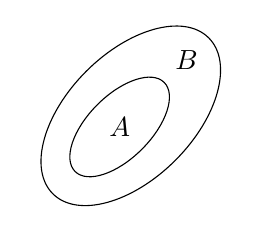
\begin{tikzpicture}[scale=0.4, line join=round, line cap=round]
			\draw[rotate=45] (0,0) ellipse (2cm and 1cm) (0,0) node{$A$}; 
			\draw[rotate=45] (0.5,0) ellipse (3.5cm and 2cm) (3,0) node{$B$}; 
	\end{tikzpicture}}
	{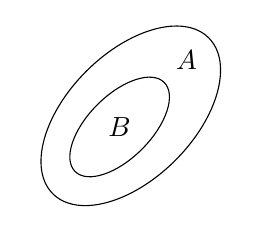
\begin{tikzpicture}[scale=0.4, line join=round, line cap=round]
			\draw[rotate=45] (0,0) ellipse (2cm and 1cm) (0,0) node{$B$}; 
			\draw[rotate=45] (0.5,0) ellipse (3.5cm and 2cm) (3,0) node{$A$}; 
	\end{tikzpicture}}
	{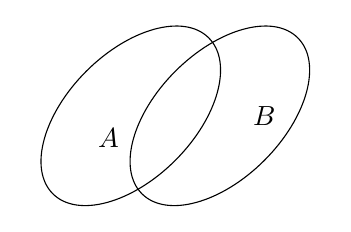
\begin{tikzpicture}[scale=0.4, line join=round, line cap=round]
			\draw[rotate=45] (0,0) ellipse (3.5cm and 2cm) (-1,0) node{$A$}; 
			\draw[rotate=45] (2,-2) ellipse (3.5cm and 2cm) (3,-3) node{$B$}; 
	\end{tikzpicture}}
	{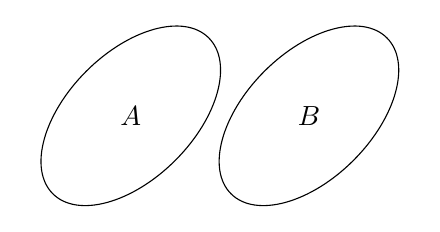
\begin{tikzpicture}[scale=0.4, line join=round, line cap=round]
			\draw[rotate=45] (0,0) ellipse (3.5cm and 2cm) (0,0) node{$A$}; 
			\draw[rotate=45] (4,-4) ellipse (3.5cm and 2cm) (4,-4) node{$B$}; 
	\end{tikzpicture}}
	\loigiai
	{
		$ A \subset B $ có biểu đồ Ven là hình vẽ:  
		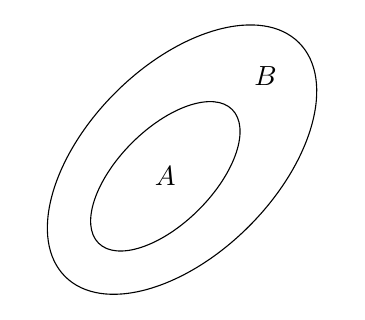
\begin{tikzpicture}[scale=0.6, line join=round, line cap=round]
			\draw[rotate=45] (0,0) ellipse (2cm and 1cm) (0,0) node{$A$}; 
			\draw[rotate=45] (0.5,0) ellipse (3.5cm and 2cm) (3,0) node{$B$}; 
		\end{tikzpicture}	
	}
\end{ex}
\begin{ex}%[0D1B3-3]
	\immini
	{
		Cho $A,B$ là hai tập hợp bất kì. Phần gạch chéo trong hình vẽ bên là tập hợp nào sau đây?
		\choice
		{$A \cup B$}
		{$B \setminus A$}
		{$A \setminus B$}
		{\True $A \cap B$}
	}
	{
		\begin{tikzpicture}[scale=0.6]
			\draw (0,0) ellipse (2cm and 1cm);
			\draw (2,0) ellipse (1.5cm and 0.7cm);
			\begin{scope}
				\clip (0,0) ellipse (2cm and 1cm);
				\fill[pattern=north west lines] (2,0) ellipse (1.5cm and 0.7cm);
			\end{scope}
			\node at (0,0) [above left] {$A$};
			\node at (2,0) [right] {$B$};
		\end{tikzpicture}
	}
	\loigiai{
	}
\end{ex}

\begin{ex}%[0D1B3-3]
	\immini{Cho tập hợp hai tập hợp $A$ và $B$ được biểu diễn bởi biểu đồ Ven như hình vẽ bên. Mệnh đề nào đúng?}{
		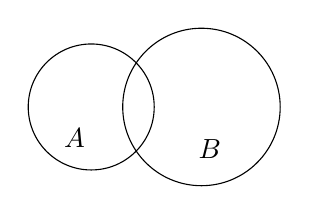
\begin{tikzpicture}[scale=.5]
			\def\radius{2cm}
			\coordinate (ceni);
			\coordinate[xshift=.7*\radius] (cenii);
			\draw (ceni) circle (.8*\radius);
			\draw (cenii) circle (\radius);
			% \draw  ([xshift=-37pt,yshift=15pt]current bounding box.north west) rectangle ([xshift=37pt,yshift=-30]current bounding box.south east);
			%\node[xshift=-.6\radius] at (ceni) {$5$};
			%\node[xshift=.7\radius] at (cenii) {$10$};
			%\node[xshift=.5\radius] at (ceni) {$10$};
			\node[xshift=-6pt,yshift=-.2*\radius] at (ceni) {$A$};
			\node[xshift=3pt,yshift=-.27*\radius] at (cenii) {$B$};
			%\node[yshift=10pt] at (current bounding box.south) {Tổng số học sinh trong lớp: $|A|=45 $};
		\end{tikzpicture}
	}
	\choice
	{$A\subset B$}
	{$A\cup B = \varnothing$}
	{\True $A\cap B \neq \varnothing$}
	{$B \subset A$}
	\loigiai
	{
		Theo biểu đồ Ven ta có $A\cap B \neq \varnothing $ là mệnh đề đúng.
	}
\end{ex}
\begin{ex}%[0D1B3-3]
	Lớp $10A5$ có $40$ học sinh, trong đó có $3$ không biết chơi cầu đá và cầu lông, biết rằng có $ 20 $ em biết chơi cầu đá và $ 13 $ em biết chơi được cầu đá và cầu lông. Hỏi lớp $ 10A5$ có bao nhiêu học sinh biết chơi cầu lông? 
	\choice
	{\True $30$}
	{$37$}
	{$17$}
	{$24$}
	\loigiai{
		\immini
		{ Ta vẽ biểu đồ Ven như hình bên.
			\begin{itemize}
				\item[•] Gọi $X$ là tập hợp các học sinh lớp $10A5$, suy ra $|X|=40$.
				\item[•] Goị $A$ là tập hợp các học sinh biết chơi cầu đá, suy ra $|A|=20$.
				\item[•] Gọi $B$ là tập hợp các học sinh biết chơi cầu lông, suy ra $|B|=?$.
			\end{itemize}	
		}
		{
			\begin{tikzpicture}[scale=.7]
				\def\radius{2cm}
				%\def\mycolorbox#1{\textcolor{#1}{\rule{2ex}{2ex}}}
				%\colorlet{colori}{blue!70}
				%\colorlet{colorii}{red!70}
				
				\coordinate (ceni);
				\coordinate[xshift=.8*\radius] (cenii);
				
				\draw (ceni) circle (\radius);
				\draw (cenii) circle (.8*\radius);
				\draw  ([xshift=-37pt,yshift=15pt]current bounding box.north west) 
				rectangle ([xshift=37pt,yshift=-30]current bounding box.south east);
				
				\node[xshift=-.6\radius] at (ceni) {$20$};
				\node[xshift=.7\radius] at (cenii) {$?$};
				\node[xshift=.5*\radius] at (ceni) {$13$};
				\node[xshift=30pt,yshift=-.7*\radius] at (ceni) {$3$};
				\node[xshift=-6pt,yshift=-.4*\radius] at (ceni) {$A$};
				\node[xshift=3pt,yshift=-.3*\radius] at (cenii) {$B$};
				\node[yshift=10pt] at (current bounding box.south) {Tổng số học sinh: $|X|=40$};
			\end{tikzpicture}
		}
		$\bullet$	Khi đó $A\cap B$ là tập hợp các học sinh biết chơi cầu đá và cầu lông, suy ra $|A\cap B|=13$.\\
		$\bullet$  $A\cup B$ là tập hợp các học sinh biết chơi cầu đá hoặc cầu lông, suy ra $|A\cup B|=?$.\\
		$\bullet$ $X\setminus (A\cup B)$ là tập hợp các học sinh không biết chơi cầu đá và cầu lông, suy ra $|X\setminus (A\cup B)| = 3$.\\
		Số học sinh biết chơi cầu đá hoặc cầu lông là
		\[|A\cup B| =|X| - |X\setminus (A\cup B)| =40 - 3=37.\]
		Số  khọc sinh biết chơi cầu lông
		\[|B|=|A\cup B| +|A\cap B|-|A| = 37+13-20=30.\]
		Vậy có $30$ học sinh biết chơi cầu lông.
	}
\end{ex}
\begin{ex}%[0D1K3-3]
	Lớp $10A$ có $42$, trong đó có $15$ học sinh giỏi Toán, $20$ học sinh giỏi Văn, trong đó $10$ học sinh giỏi cả Toán và Văn. Hỏi có bao nhiêu học sinh không giỏi cả Toán và Văn?
	\choice
	{\True $ 17 $}
	{$25$}
	{$5$}
	{$10$}
	\loigiai{
		\immini
		{ Ta vẽ biểu đồ Ven như hình bên.
			\begin{itemize}
				\item[•] Gọi $X$ là tập hợp các học sinh lớp $10A$, suy ra $|X|=42$.
				\item[•] Goị $A$ là tập hợp các học sinh giỏi Toán, suy ra $|A|=15$.
				\item[•] Gọi $B$ là tập hợp các học sinh giỏi Văn, suy ra $|B|=20$.
			\end{itemize}	
		}
		{
			\begin{tikzpicture}[scale=.7]
				\def\radius{2cm}
				%\def\mycolorbox#1{\textcolor{#1}{\rule{2ex}{2ex}}}
				%\colorlet{colori}{blue!70}
				%\colorlet{colorii}{red!70}
				
				\coordinate (ceni);
				\coordinate[xshift=.8*\radius] (cenii);
				
				\draw (ceni) circle (\radius);
				\draw (cenii) circle (.8*\radius);
				\draw  ([xshift=-37pt,yshift=15pt]current bounding box.north west) 
				rectangle ([xshift=37pt,yshift=-30]current bounding box.south east);
				
				\node[xshift=-.6\radius] at (ceni) {$15$};
				\node[xshift=.7\radius] at (cenii) {$20$};
				\node[xshift=.5*\radius] at (ceni) {$10$};
				\node[xshift=-6pt,yshift=-.4*\radius] at (ceni) {$|A|$};
				\node[xshift=3pt,yshift=-.3*\radius] at (cenii) {$|B|$};
				\node[yshift=10pt] at (current bounding box.south) {Tổng số học sinh: $|X|=42$};
			\end{tikzpicture}
		}
		$\bullet$ Khi đó $A\cap B$ là tập hợp các học sinh giỏi cả Toán và Văn, suy ra $|A\cap B|=10$.\\
		$\bullet$ $A\cup B$ là tập hợp các học sinh giỏi Toán hoặc Văn.\\
		$\bullet$  $X\setminus (A\cup B)$ là tập hợp các học sinh không giỏi Toán và Văn.\\
		Số học sinh giỏi Toán hoặc Văn là
		\[|A\cup B| = |A|+|B|-|A\cap B|=15+20-10=25.\]
		Số  không giỏi Toán và Văn là
		\[|X\setminus (A\cup B)|=|X|-|A\cup B| =42-25=17.\]
		Vậy có $17$ học sinh không giỏi Toán và Văn.
	}
\end{ex}
\begin{ex}%[0D1K3-3]
	Lớp $ 10A $ có $ 45 $ học sinh, trong đó có $ 15 $ học sinh được xếp loại học lực giỏi, $ 20 $ học sinh được xếp loại hạnh kiểm tốt, $ 10 $ em vừa xếp loại học lực giỏi, vừa có hạnh kiểm tốt. Hỏi có bao nhiêu học sinh xếp loại học lực giỏi hoặc có hạnh kiểm tốt?
	\choice
	{\True $ 25 $}
	{$ 10 $}
	{$ 45 $}
	{$ 35 $}
	\loigiai{
		\immini
		{
			Đáp án A đúng vì: Gọi $ A $ là tập hợp học sinh lớp 10A; $ B $ là tập hợp học sinh có học lực giỏi; $ C $ là tập hợp các học sinh có hạnh kiểm tốt. Khi đó tập hợp cần tìm là tập $ B \cup C $. Tập này có $ 25 $ học sinh. Được thể hiện trong biểu đồ Ven như sau:\\
			Đáp án B sai vì học sinh tính nhầm $ A \cup B $.\\
			Đáp án C sai vì học sinh cộng lại: $ 15+20+10=45 $.\\
			Đáp án D sai nhầm tính $ 15+20=35 $.
		}
		{
			\begin{tikzpicture}[scale=.8]
				\def\radius{2cm}
				%\def\mycolorbox#1{\textcolor{#1}{\rule{2ex}{2ex}}}
				%\colorlet{colori}{blue!70}
				%\colorlet{colorii}{red!70}
				
				\coordinate (ceni);
				\coordinate[xshift=.7*\radius] (cenii);
				
				\draw (ceni) circle (.8*\radius);
				\draw (cenii) circle (\radius);
				\draw  ([xshift=-37pt,yshift=15pt]current bounding box.north west) 
				rectangle ([xshift=37pt,yshift=-30]current bounding box.south east);
				
				\node[xshift=-.6\radius] at (ceni) {$5$};
				\node[xshift=.7\radius] at (cenii) {$10$};
				\node[xshift=.5\radius] at (ceni) {$10$};
				\node[xshift=-6pt,yshift=-.5*\radius] at (ceni) {$B$};
				\node[xshift=3pt,yshift=-.67*\radius] at (cenii) {$C$};
				\node[yshift=10pt] at (current bounding box.south) {Tổng số học sinh trong lớp: $|A|=45 $};
			\end{tikzpicture}
		}
	}
\end{ex}
\begin{ex}%[0D1K3-3]
	Một lớp có $ 45 $ học sinh. Mỗi em đều đăng ký chơi ít nhất một trong hai môn: bóng đá và bóng chuyền. Có $ 35 $ em đăng ký môn bóng đá, $ 15 $ em đăng ký môn bóng chuyền. Hỏi có bao nhiêu em đăng ký chơi cả $ 2 $ môn?
	\choice
	{\True $ 5 $}
	{$ 10 $}
	{$ 30 $}
	{$ 25 $}
	\loigiai{
		\immini
		{
			Đáp án A đúng vì: Gọi $ A $ là tập hợp các học sinh đăng ký chơi bóng đá, $ B $ là tập hợp các học sinh đăng ký chơi bóng chuyền. Dựa vào biểu đồ Ven, ta có: số học sinh đăng ký cả $ 2 $ môn là $ |A \cap B|=|A|+|B|-|A \cup B|=35+15-45=5 $.\\
			Đáp án B sai vì học sinh tính $ 45-35=10 $.\\
			Đáp án C sai vì học sinh tính $ 45-15=30 $.\\
			Đáp án D sai vì học sinh tính $ (35+35):2=25 $.
		}
		{
			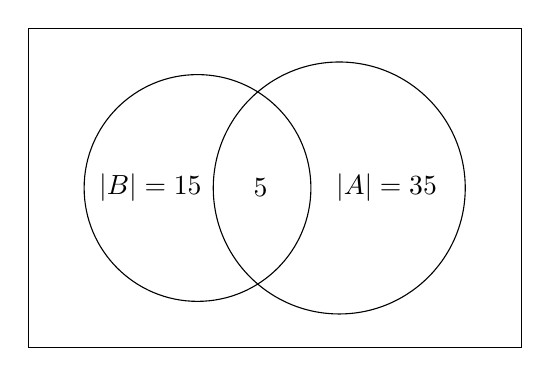
\begin{tikzpicture}[scale=.8]
				\def\radius{2cm}	
				\coordinate (ceni);
				\coordinate[xshift=.9*\radius] (cenii);
				
				\draw (ceni) circle (.9*\radius);
				\draw (cenii) circle (\radius);
				\draw  ([xshift=-25pt,yshift=15pt]current bounding box.north west) 
				rectangle ([xshift=25pt,yshift=-15]current bounding box.south east);
				
				\node[xshift=-.3*\radius] at (ceni) {$|B|=15$};
				\node[xshift=.3*\radius] at (cenii) {$|A|=35$};
				\node[xshift=.4*\radius] at (ceni) {$5$};
			\end{tikzpicture}
		}
	}
\end{ex}
\begin{ex}%[0D1K3-3]
	Lớp $ 10B $ có $ 45 $ học sinh, trong đó có $ 25 $ em thích môn Văn, $ 20 $ em thích môn Toán, $ 18 $ em thích môn Sử, $ 6 $ em không thích môn nào, $ 5 $ em thích cả ba môn. Hỏi số em thích chỉ một trong ba môn là bao nhiêu?
	\choice
	{\True $ 20 $}
	{$ 30 $}
	{$ 15 $}
	{$ 25 $}
	\loigiai{
		\immini
		{
			Ta vẽ biểu đồ Ven như hình bên.\\
			Gọi $ a,b,c $ theo thứ tự là số học sinh chỉ thích môn Văn, Sử, Toán.\\
			$ x $ là số học sinh chỉ thích hai môn là Văn và Toán.\\
			$ y $ là số học sinh chỉ thích hai môn là Sử và Toán.\\
			$ z $ là số học sinh chỉ thích hai môn là Văn và Sử.\\
			Ta có số em thích nhất một môn là $ 45-6=39 $.\\
			Dựa vào sơ đồ Ven ta có phương trình:\\
			$(I)
		\heva{
			&	a+x+z+5=25\\
			&	b+y+z+5=18\\
			&	c+x+y+5=20\\
			&	x+y+z+a+b+c+5=39
			}$
		}
		{
			\begin{tikzpicture}[scale=.8]
				\def\radius{2cm}	
				\coordinate (ceni);
				\coordinate[xshift=.8*\radius] (cenii);
				\coordinate[xshift=.4*\radius,yshift=-.8*\radius] (ceniii);
				\draw (ceni) circle (.9*\radius);
				\draw (cenii) circle (\radius);
				\draw (ceniii) circle (1.1*\radius);
				
				\node[xshift=-1.05*\radius,yshift=.2*\radius] at (ceni) {$18$ (Sử)};
				\node[xshift=-.3*\radius, yshift=.2*\radius] at (ceni) {$b$};
				\node[xshift=.35*\radius, yshift=.3*\radius] at (ceni) {$y$};
				\node[xshift=-.1*\radius, yshift=-.45*\radius] at (ceni) {$z$};
				\node[xshift=.35*\radius, yshift=-.25*\radius] at (ceni) {$5$};
				
				\node[xshift=1.3*\radius] at (cenii) {$20$ (Toán)};
				\node[xshift=.1*\radius, yshift=-.5*\radius] at (cenii) {$x$};
				\node[xshift=1.1*\radius,yshift=.2*\radius] at (ceni) {$c$};
				\node[xshift=1.3*\radius, yshift=-.2*\radius] at (ceniii) {$25$ (Văn)};
				\node[yshift=-.4*\radius] at (ceniii) {$a$};
			\end{tikzpicture}
		}
		\noindent Giải hệ phương trình $ (I) $ bằng cách cộng vế với vế $ 3 $ phương trình đầu ta có: \\$ a+b+c+2(x+y+z)+15=63 $\\
		kết hợp với phương trình cuối của hệ: $ x+y+z+a+b+c+5=39 $ ta được:\\
		$ a+b+c+2(39-5-a-b-c)+15=63 \Rightarrow a+b+c=20 $.\\
		Vậy chỉ có $ 20 $ em thích chỉ một môn trong ba môn trên.
	}
\end{ex}

%%=====Câu 1
\begin{ex}%[0D1B3-4]
	Cho số thực $a<0$. Điều kiện cần và đủ để $(-\infty ; 9a) \cap \left( {\dfrac{4}{a};+\infty}\right)  \neq  \varnothing$ là
	\choice
	{\True $-\dfrac{2}{3}<a<0$}
	{$-\dfrac{2}{3}\leq a<0$}
	{$-\dfrac{3}{4}<a<0$}
	{$-\dfrac{3}{4}\leq a<0$}
	\loigiai{%A
		Điều kiện thỏa đề bài $9a > \dfrac{4}{a} \Leftrightarrow a^2 < \dfrac{4}{9}  \Leftrightarrow \left| {a}\right| < \dfrac{2}{3} \Leftrightarrow -\dfrac{2}{3}<a<0$.
	}
\end{ex}

%%=====Câu 2
\begin{ex}%[0D1B3-4]
	Với giá trị nào của $m$ thì $(m-7;m)\cap (-4;3)=(m-7;m)$?
	\choice{$m\in \varnothing $}
	{$m<3 $}
	{\True $m=3 $}
	{$ m>3$}
	\loigiai{
	Ta có\\
		$(m-7;m)\cap (-4;3)=(m-7;m)\Leftrightarrow(m-7;m)\subset (-4;3) \Leftrightarrow \heva{&m-7\ge -4 \\ & m \le 3} \Leftrightarrow \heva{&m \ge 3 \\ & m \le 3} \Leftrightarrow m = 3$.
	}
\end{ex}

%%=====Câu 3
\begin{ex}%[0D1B3-4]
	Cho hai tập hợp $A=[m+1;m+4]$ và $B=(-\infty;5)$. Tìm tất cả các giá trị của $m$ để $A \cap B=\varnothing$.
	\choice
	{$m<4$}
	{\True $m\geq 4$}
	{$m>4$}
	{$m\leq 4$}
	\loigiai{
		Ta có $A\cap B=\varnothing\Leftrightarrow m+1\geq 5\Leftrightarrow m\geq 4$.}
\end{ex}

%%=====Câu 4
\begin{ex}%[0D1B3-4]
	Cho hai tập hợp $A = (-3; 2]$ và $B = [m; m + 1)$. Tìm tất cả các giá trị của $m$ để $A \cap B=\varnothing$
	\choice
	{\True $m \in (-\infty;-4]\cup (2;+\infty)$}
	{$m \in (-4;2)$}
	{$m \in (-4;2]$}
	{$m \in [-4;2)$}
	\loigiai{
		Ta có
		\[A\cap B=\varnothing\Leftrightarrow \hoac{&m> 2\\ &m+1\le -3}\Leftrightarrow \hoac{&m> 2\\ &m\le -4}\Leftrightarrow m\in (-\infty;-4]\cup (2;+\infty).\]
	}
\end{ex}

%%=====Câu 5
\begin{ex}%[0D1B3-4]
	Cho tập hợp $A=\left[m; m+1\right]$, $B=[1; 3]$. Tập hợp tất cả các giá trị của $m$ để $A\subset B$ là
	\choice
	{$m\le 1$ hoặc $m\ge 2$}
	{\True $1\le m\le 2$}
	{$1<m<2$}
	{$0\le m\le 2$}
	\loigiai{
		Để $A\subset B$ thì $\heva{
			& m\ge 1 \\
			& m+1\le 3} \Leftrightarrow 1\le m\le 2$.
	}
\end{ex}

%%=====Câu 6
\begin{ex}%[0D1B3-4]
	Cho $A=(2;+\infty)$, $B=(m;+\infty)$. Điều kiện cần và đủ của $m$ sao cho $B$ là tập con của $A$ là
	\choice
	{$m\leqslant 2$}
	{$m=2$}
	{$m>2$}
	{\True $m\geqslant 2$}
	\loigiai{
		Ta có $B\subset A$ khi và chỉ khi $\forall x\in B \Rightarrow x\in A$ $ \Rightarrow m\geqslant 2$.
		\begin{center}
			\begin{tikzpicture}
				\draw[->](-2,0)->(4,0);
				\IntervalLR{-2}{2}
				\def\skipInterval{0.5cm}%Khoảng cách đặt nhãn
				\IntervalGRF{}{}{\big)}{2}%Gạch xọc phải qua trái
			\end{tikzpicture}
		\end{center}
	}
\end{ex}

\Closesolutionfile{ans}